%!TeX spellcheck = en-GB
\documentclass[12pt,a4paper]{report}

\usepackage[utf8]{inputenc}
\usepackage[english]{babel}
\usepackage{titling}
\usepackage{array}
\usepackage{amsmath}
\usepackage{epstopdf}
\usepackage{graphicx}
\usepackage{subcaption}
\usepackage{float}
\usepackage{placeins}
\usepackage{wrapfig}
\usepackage{diagbox}
\usepackage{hyperref}
\usepackage{pbox}
\usepackage{fancyhdr}
\usepackage[a4paper]{geometry}
\usepackage{header}
\usepackage[absolute,overlay]{textpos}
  \setlength{\TPHorizModule}{1mm}
  \setlength{\TPVertModule}{1mm}
  
  \usepackage[toc,page]{appendix}
  
\usepackage{listings}
\usepackage{color}
 
\definecolor{codegreen}{rgb}{0,0.6,0}
\definecolor{codegray}{rgb}{0.5,0.5,0.5}
\definecolor{codepurple}{rgb}{0.58,0,0.82}
\definecolor{backcolour}{rgb}{0.95,0.95,0.92}
 
\lstdefinestyle{mystyle}{
    backgroundcolor=\color{backcolour},   
    commentstyle=\color{codegreen},
    keywordstyle=\color{magenta},
    numberstyle=\tiny\color{codegray},
    stringstyle=\color{codepurple},
    basicstyle=\footnotesize,
    breakatwhitespace=false,         
    breaklines=true,                 
    captionpos=b,                    
    keepspaces=true,                 
    numbers=left,                    
    numbersep=5pt,                  
    showspaces=false,                
    showstringspaces=false,
    showtabs=false,                  
    tabsize=2
}
\lstset{style=mystyle}

\usepackage[show]{chato-notes} % change the "show" option to "hide" to remove all \todo and \note blocks


\geometry{hscale=0.8,vscale=0.8,centering}
\fancyhf{}
\fancyhead[L]{}
\fancyhead[R]{}
\cfoot{\thepage}
\setlength{\droptitle}{-6em}

\newcommand{\blap}[1]{\vbox to 0pt{#1\vss}}
\newcommand\AtUpperLeftCorner[3]{%
  \put(\LenToUnit{#1},\LenToUnit{\dimexpr\paperheight-#2}){\blap{#3}}%
}
\newcommand\AtUpperRightCorner[3]{%
  \put(\LenToUnit{\dimexpr\paperwidth-#1},\LenToUnit{\dimexpr\paperheight-#2}){\blap{\llap{#3}}}%
}

\newcommand\AtDownRightCorner[3]{%
  \put(\LenToUnit{\dimexpr\paperwidth-#1},\LenToUnit{#2}){\blap{\llap{#3}}}%
}

\newcommand{\HRule}{\rule{\linewidth}{0.5mm}}

\title{PROJ0011-1 Personal student project}
\subTitle{Integration of libopencm3 in FreeRTOS for stm32f4 and stm32f3 MCU}
\author{Pierre Nicolay}
\acYear{2018-2019}
\univ{University of Liège}
\date{\today}
\makeatletter

\begin{document}

\begin{titlepage}
  \begin{textblock}{30}(150,20)
      
\includegraphics[width=4cm]{Headers/ulg.png}
  \end{textblock}
  \begin{textblock}{30}(125,240)
      
\includegraphics[width=9.0cm]{Headers/facsa.png}
  \end{textblock}
  \hbox{
  \hspace*{0.2\textwidth}
  \rule{1pt}{\textheight}
  \hspace*{0.05\textwidth}
  \parbox[b]{0.75\textwidth}{ % P
  \begin{flushleft}
    {\noindent\Huge\bfseries \@title}\hspace*{0.2\textwidth}
    \\\HRule\\[2\baselineskip]
    {\Large \textsc{\@subTitle}}\\[4\baselineskip]
    {\large \textsc{\@author}}\\[2\baselineskip]
    {\large \textsc{\@univ: }}
    {\large \textsc{\@acYear}}\\[20\baselineskip]
    \@date
  \end{flushleft}
  \vspace*{0.05\textheight}
  \hspace*{0.3\textwidth}
  }}

\end{titlepage}

\tableofcontents
\listoffigures
\lstlistoflistings

\newpage
\chapter{Introduction}
\label{ch:intro}
This project lies in the scope of the \emph{RoboCupSoccer competition} project. For readers already familiar with this competition, we invite them to skip the introduction and pursue their reading at chapter \ref{ch:prob}.\newline
The Robocup competition is an international science and technology tournament created in 1997 \cite{robocupHistory}. The goal is to promote technology and to advance the state-of-the-art in robotic and AI through a landmark project such as robots playing soccer. However the ultimate goal is the following: \newline ``by the middle of the 21st century, a team of fully autonomous humanoid robot soccer players shall win a soccer game, complying with the official rules of FIFA, against the winner of the most recent World Cup.'' \cite{RobocupObjective}.\newline
The university of liege made up a team to take part in the competition. The category we want compete in is the \emph{Humanoid kidSize}. In contrast to the \emph{Standard Platform}, the \emph{Humanoid kidSize} doesn't provide a platform. Therefore we first needed to build a robotic platform. The platform illustrated in figure \ref{fig:platform} is composed of joint and links. 
\begin{figure}[h]
  \begin{minipage}[c]{0.3\textwidth}
    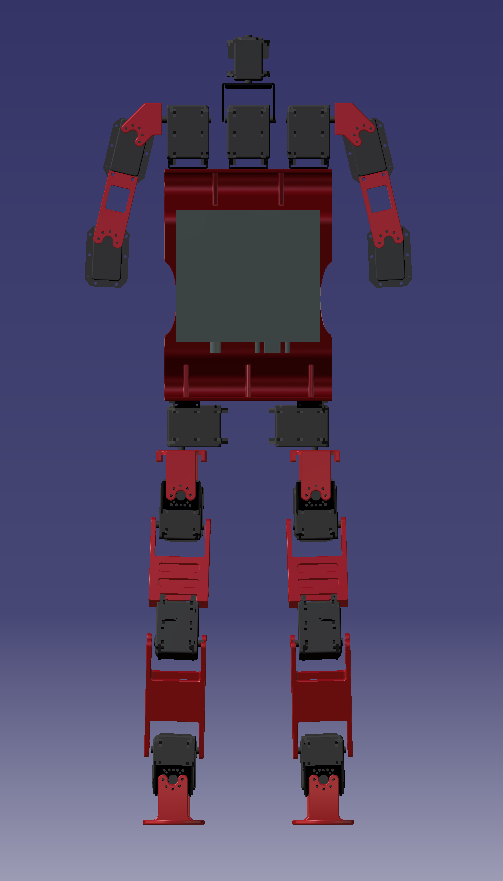
\includegraphics[width=\textwidth]{figs/platform.png}
  \end{minipage}\hfill
  \begin{minipage}[c]{0.6\textwidth}
    \caption{Illustration of our platform. Each joint, in black, is a servo motor (MX-28 \cite{MX28}) and each link, in red, is a 3D printed segment linking every joint together. The choice of this design is not discussed here. Some part of the design explanation can be found in 
    \cite{VanLaeken}'s work. This document is not publicly available, an interested reader can email at \cite{VanLaeken} \href{mailto:Lionel.vanlaeken@student.uliege.be}{Lionel.vanlaeken@student.uliege.be} to get the document. We do not have more documents to present.}
    \label{fig:platform}
  \end{minipage}
\end{figure}
This project is focused on the low-level software implementation needed to drive every servo motor. 
The origin of this project comes out of \cite{masterGL}'s work. \cite{masterGL} proposed to change the internal electronic components of every servo in order to, among others:
\begin{itemize}
\item increase the control accuracy.
\item easily implement a variety of handcrafted commands.
\item implement more accurate sensors.
\item enable communication through CAN bus.
\item use of a more powerful microcontroller.
\end{itemize}
The next logical part of the work is thus to add a software layer in order to use the new homemade board's feature.\newline
The goal of this project is to implement a software layer using a real time operating system (RTOS) as well as enabling USB communication supported by the MCU.\newline
This document's purpose is twofold. On one hand, defining the problem and explaining the solution used to solve it. On the other hand, giving a documentation and a starting point for the \emph{uLiege robocup}'s team members in order to continue the project.\newline
This project was developed on Ubuntu 16.04 LTS with board stm32f429i-discovery and\\ stm32f3dicovery. Thus we can only ensure compilation and testing on those platform. There might be some extra work for other development platform.\newline
In the next chapter we are going to define the problem we are facing and how it relates to the \emph{RoboCupSoccer competition} project.\newpage
\chapter{Problem Statement}
\label{ch:prob}
As mentioned previously, the goal of the project is mainly to use a RTOS along with a MCU firmware. The MCUs used on \cite{masterGL}'s board are part of the stm32f3 family. In addition to this, we also needed to handle the stm32f4 family. The reason for this is that an other board is currently being developed by \emph{uLiege robocup}'s team. It will be equiped with a processor of the stm32f4 type.\newline
As we would like to communicate with different devices over a USB communication as well as drive the servo motors or even monitor every sensor we decided before beginning of the project to use a RTOS.\newline
The utility of the RTOS is multiple. First, it gives the programmer a comfortable programming work-frame for inter-process communication, by providing tools such as semaphores, mutex, message Queues, software timers, etc. In addition to this the RTOS provides a consistency concerning the execution time of each task.\newline
The RTOS chosen here is FreeRTOS. More details can be found in section~\ref{sec:freeRTOS}. We also needed a firmware to interact with the different functionalities of the MCU. The library chosen, despite the existence of the vendor's one, is \emph{Libopencm3} (section~\ref{sec:libopencm3}). 
\chapter{Libraries and toolchain}

This chapter gives useful information about the different libraries used in this project. First a description of the library followed by a discussion on the support and a evaluation of the library. A following chapter \ref{chap:impl} will give implementation details of the project as well as a description of main function used and their explanation. A final Chapter \ref{chap:doc} will give tips and hints and a documentation for student willing to pursue the work. This chapter also contains information about the toolchain used to compile and flash the code on the MCUs.
\section{Libopencm3}

\label{sec:libopencm3}
Libopencm3 (\cite{cm3}) is a ``Open-Source low level hardware library for ARM Cortex-M3 micro-controllers (but also M0, M4 are supported and more to come)''. It aims at creating a open-source firmware library supporting a lot of ARM-cortex-M3 MCU. Even though we are aware of the STM32Cube~\cite{cube}, we opt for libopencm3 for multiple reasons. At first, it is an open-source and a well maintained library under version 3 of the GNU General Public License. Secondly, STM32Cube provides a hardware abstraction layer (HAL) that provides a simple and easy to use API which  is portable on different STM32 MCU. To build this abstraction, they needed to add a lot of software layers, resulting into a too inefficient library four our needs. They also provided a low-level (LL) API, howver it is too expert oriented. In contrast to this, libopencm3's code is not immediately portable across different cortex MCUs, however this results in a light-wise, way more efficient API than HAL. But also more easy to use than LL.\newline
One downside in using Libopencm3 is that it is currently a work in progress. It is therefore not considered stable for every processor in addition to a non stable API, function names and macro could be changed at any time without warning.\newpage
\section{FreeRTOS}

\label{sec:freeRTOS}
This section will describe FreeRTOS \cite{FreeRTOSBook}. FreeRTOS kernel is a free to use and the market-leading RTOS. It is designed to be simple and easy to use. Only 3 kernel files and 1 portable, controller dependant, source file are needed to run FreeRTOS on a MCU. There are many other reasons to chose FreeRTOS. It is under open-source MIT license and fully supported. It is known to be stable as well as widely used, resulting in a very active supporting forum. It is also very small, generally leading to a 6K up to 12K bytes binary image. In addition to this it is given with a lot of example application for each supported port. The stm32f3 and stm32f4 are part of the supported family. Finally FreeRTOS is very scalable and ``FreeRTOS offers a smaller and easier real time processing alternative for applications where eCOS, embedded Linux (or Real Time Linux) and even uCLinux won't fit, are not appropriate, or are not available''.\newline
For all those reasons we decide to use FreeRTOS.

\section{Arm-none-eabi}
In order to compile the code into an understandable set of instructions for the stm32f4 and f3 MCU families, we used the GNU Embedded Toolchain of Arm \cite{arm}. This toolchain targets ARM cortex-M families of processor, it is open-source and includes the GNU compiler. The version used in this project is arm-none-eabi 7.3.1. This version is not immediately available on the APT repositories of Ubuntu. In order to use it one need to download the source code on the vendor website, build it and install it. The building and installing instruction are given with the source code. We do not ensure compilation for a version lower than this one.

\section{Openocd}
Finally we needed a way to flash the compiled code to the processor's flash memory. To do so we used OpenOCD \cite{hoglAbstractopen}. OpenOCD (open on chip debugger) is an open-source JTAG debugger for ARM processor family. Even though flashing the chip is not the first purpose of openOCD, it is however possible and is is also the solution used in this project.
\chapter{USB}
\label{chap:usb}
This chapter will introduce USB communication. It is mostly useful for students pursuing this work as most of them are unfamiliar with this protocol. We will thus describe how to program a software USB
device thanks to \cite{usb-explained}.\newline
First in order to understand USB communication one need to understand the difference between the host and the devices. USB communication contains only one host and multiple connected devices. The host initiates all traffic. At initialization, the device identifies itself to the host by sending a \emph{device descriptor} and a \emph{configuration descriptor}. Those descriptor indicates the host about the capabilities of the device. In particular, the \emph{configuration descriptor} includes the number on interfaces available on a device. An USB interface defines a device specific function.\newline To get a better understanding of a USB interface one could imagine the following example. For our servo motor device, we could have multiple interfaces. For example one interface allowing to drive the motor, another interface for a specific sensor on the board, allowing us to retrieve the different sensor values from the device.\newline
Every interface on a USB device is composed of multiple endpoints. Endpoints are communication channels and are defined with respect to the host. This is very important to understand in order to correctly implement a USB device.\newline
An \emph{IN} endpoint sends data from the device to the host whereas an \emph{OUT} endpoint transfers data from the host to the device. Endpoints are numbered between 0 and 15.\newline
According to USB.org, there are 4 types of endpoint.
\begin{itemize}
    \item Bulk endpoints. Those endpoints are analog to the TCP/IP protocol where every send package needs to be acknowledged. It is reliable and fault-tolerant.
    \item Isochronous endpoints. They are used to transport real-time data. ``A fixed bandwidth is allocated to them. The host allocates this bandwidth and will not allow an isochronous endpoint to be created if no bandwidth is available. In contrast, bulk endpoints have no guaranteed bandwidth.''
    \item Control endpoints is a mandatory endpoint numbered 0 used for general operations such as sending the \emph{descriptors} or even changing different device's parameters such as the baud rate or the packet volume.
    \item Interrupt endpoints. Those endpoints ``are polled occasionally by the host and enable a device to report status changes.''
\end{itemize}
As mentioned in \cite{usb-explained} USB traffic is organized in frames. Every frame is initiate every 125 $\mu s$ (for high speed USB communication) by the host sending a start of frame. ``Isochronous endpoints are allocated a transfer in every frame packet. Interrupt endpoints are polled once every so many frames, and bulk transfers may happen anytime when the bus is not in use.''\newline
As mentioned earlier, when a device is plugged in the bus, the host request the \emph{device descriptors}. The descriptor provides 2 pieces of useful information, the device's class as well as the vendorID/productID (VID/PID). The class of the device is specified by the programmer and can be of any type defined by USB.org. For example, a keyboard connected through USB would have a human interface device (HID) class. If no class defined by USB.org is suitable for a device, one can create his own class.\newline
In the case of a device complying with USB specific device class, the host will have the generic driver in order to pilot your device. In the other case where no USB.org specific class is suitable for your application, you need to define the class as \emph(vendor-specific). The host will then use the VID/PID to find the corresponding driver.\newline
\chapter{Implementation details}
\label{chap:impl}
This chapter focuses on the explanation of the project. First we will describe the structure of the project. Then we will present every application in order of their development. We invite the reader to read this alongside with the code, and try out the different applications in order to get familiar with libopencm3 and FreeRTOS.\newline The code is available on uLiege's git repository. 
\paragraph{Remark} If there is any trouble compiling/flashing or error during the execution the reader should first start looking at section \ref{sec:trouble} for some guidance.\newline
\noindent The directory the reader is interested in, is located at :
\begin{lstlisting}[language=bash]
$ cd /<path-to-repo>/robocup/electronique/code/src/stm23f4/
\end{lstlisting}
Most of the work of this section is an adaptation of \cite{Gay2018}'s work. 
\section{Directory Structure and compilation}
The directory's structure is showed in \ref{fig:dir}.

\begin{wrapfigure}{r}{0.45\textwidth}
  \vspace{-20pt}
  \centering
  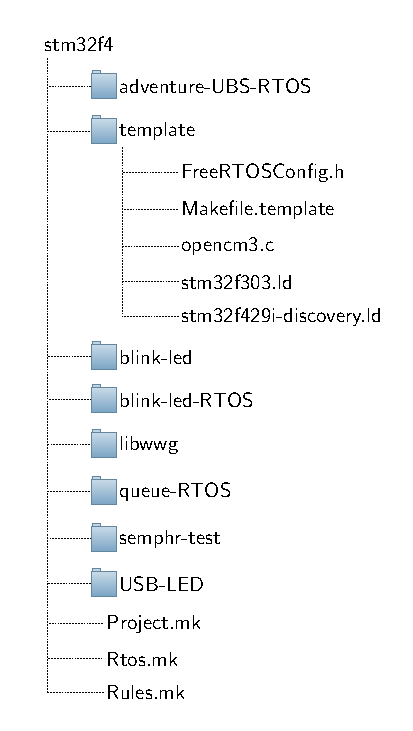
\includegraphics[width=0.30\textwidth]{figs/tree.pdf}
  \vspace{-10pt}
  \caption{Directory structure}
  \vspace{-118pt}
  \label{fig:dir}
\end{wrapfigure}
The most important folder for someone wanting to create a new project is the template folder. It contains all the necessary file in order to create a new project. Instruction on the creation of a new project can be found in chapter \ref{chap:doc}.
To build and run a project, one simply run "make" from a given application folder. However before trying to build any project, one need to build Libopencm3 and libwwg (only for application using USB). To build liopencm3 you need to run:

\begin{lstlisting}[language=bash]
$ cd /<path-to-repo>/robocup/electronique/code/libopencm3
$ make
\end{lstlisting}
To build libwwg you run: 
\begin{lstlisting}[language=bash]
$ cd /<path-to-repo>/robocup/electronique/code/src/stm23f4/libwwg
$ make
\end{lstlisting}
This library is formatting the message according to minicom's format among with other functionalities. This library was written by \cite{Gay2018} but is not documented. You need to read the source code to understand it's utility.
Once this is done, you go into the directory of the desired application and run:
\begin{lstlisting}[language=bash, label=code:f4]
$ make flash
\end{lstlisting}
for stm32f4 processor or run:
\begin{lstlisting}[language=bash, label=code:f3]
$ make ARCH=F3 flash
\end{lstlisting}
for stm32f3 processor.

\section{Blink-led}
\label{sec:bl}
This first application is very simple but illustrates how easy it is to write a blink led program using libopencm3 (only written for stm32f4 processor). It is composed of only a few set of instructions~\ref{code:blink}. First we initialize the clock of the MCU. This is done at line 5. This instruction sets the clock to $168MHz$. There are other frequency available and can be found in libopencm3's documentation. Line 10 enables the clock for the GPIO port containing the desired led. The final initialization part requires us to set the LED GPIO pin as an output port (line 12).\newline
The final interesting instruction of this file is the $gpio\_toggle$ instruction. This instruction allows us to toggle a GPIO pin. 
One downside of this application is implied by the 2 for loops. Those 2 loops slow down the blinking of the led to be perceptible by a human eye. They however prevent the processor to execute other task while waiting. On could want to use hardware timers and trigger interrupts, allowing the processor to execute useful instruction in the mean time. In the next section we will see how this can be done, without hardware timers but with a RTOS and the software timers API provided.
\section{Blink-led-RTOS}
\label{sec:blr}
The next application has exactly the same goal as the one before, however we make use of FreeRTOS allowing us to use multitasking with software Timers. This will allow us to suspend a task, give the processor to other tasks until the end of the timer, which will resume the task. The configuration of freeRTOS is the same in every application and will be explained in chapter \ref{chap:doc}. There are 2 main differences between this project and the previous one. First, the loops present in \ref{sec:bl} are replaced with the call to the FreeRTOS software timer function (line 4 \ref{code:t1}). Secondly, we create 2 FreeRTOS tasks in line 14 and 20 of \ref{code:m1}. Those 2 tasks are launched with the call to the RTOS scheduler (line 27 \ref{code:m1}). The two tasks run in parallel (from the view point of the user) and do not communicate with one another. The next application will demonstrate how we can implement tasks communication with the help of FreeRTOS tools. 
\section{Queue-RTOS}
\label{sec:qr}
This application's purpose is to illustrate how two FreeRTOS tasks can communicate as well as passing arguments to a task. This is showed thanks to message queue. To implement this application we made use of some features available on the stm32f429i-discovery development board \ref{fig:board}. This board is equipped with a user button. This button (in blue in figure~\ref{fig:board}) is connected to a GPIO port. We will thus implement 3 tasks. 1 task to blink a led, it is independent of the 2 other tasks. A second task that listens to the button and notifies the 3rd task whenever the user presses the button. Finally a 3rd task that toggles a led whenever the button is pressed.\newline
The first task is exactly the same as the one in \ref{code:t1}. The 2 other tasks are showed in \ref{code:t2}. The listening task (line 1 to 16 \ref{code:t2} first gets the message queue passed as argument. Then it listens to the button port. Lines 9 to 12 handle the button's bounces. A better way to implement this would be to remove line 6 and implement this task as a ISR, triggered when the button is pressed. We leave this to a future work. Once the button is pressed, the task puts a value in the message queue. The receiving part starts at line 18 up to line 21 \ref{code:t2}. The important instruction is line 25. This instruction listens to the queue. With our configuration of FreeRTOS, this instruction blocks the task while the queue is empty.\newline
File \ref{code:m2} shows how to initiate the message queue (line 13-16) and how to pass it as argument to a task (line 28 and 34). 
\begin{figure}[h]
    \centering
    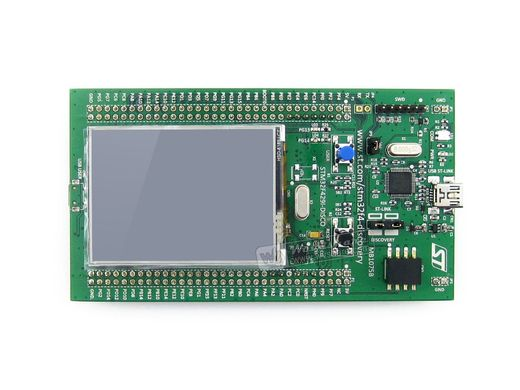
\includegraphics[scale=0.5]{figs/board.jpg}
    \caption{Development board for the stm32f4 mcu.}
    \label{fig:board}
\end{figure}
\section{Adventure-RTOS}
\label{sec:ar}
This application is the first application that uses USB communication. It is an adaptation of \cite{adventure}'s work. This work is adapted in order to communicate through USB. In order to play the game, the user need to install minicom, an old terminal program.\newline
\paragraph{Minicom setup.} To use minicom correctly with the application, you first need to set it up correctly. To do so, run 
\begin{lstlisting}[language=bash]
$ minicom -s
\end{lstlisting}
From \ref{fig:miniSetup} go to option "Serial port setup". Then press "A" to set the Serial device name. The name should be "/dev/ttyAMC0" (on a mac you can try "/dev/cu/ttyAMC0"). Once this is done, you can set the port parameter to "38400 8N1" by typing in "E" then "D" and "Q". As we will keep this configuration across multiple application, you can save this configuration.
\begin{figure}[H]
    \centering
    \begin{subfigure}[b]{0.3\textwidth}
        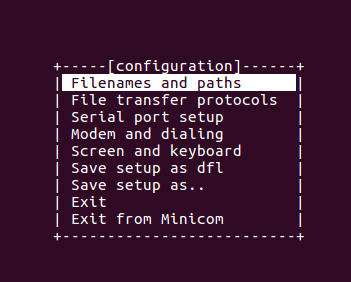
\includegraphics[width=\textwidth]{figs/minicom.png}
        \caption{Minicom setup}
        \label{fig:miniSetup}
    \end{subfigure}
    ~
    \begin{subfigure}[b]{0.3\textwidth}
        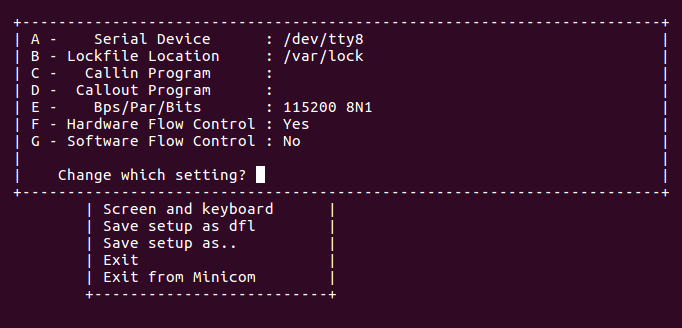
\includegraphics[width=\textwidth]{figs/serialPort.png}
        \caption{Serial port setting}
        \label{fig:serial}
    \end{subfigure}
    ~
    \begin{subfigure}[b]{0.3\textwidth}
        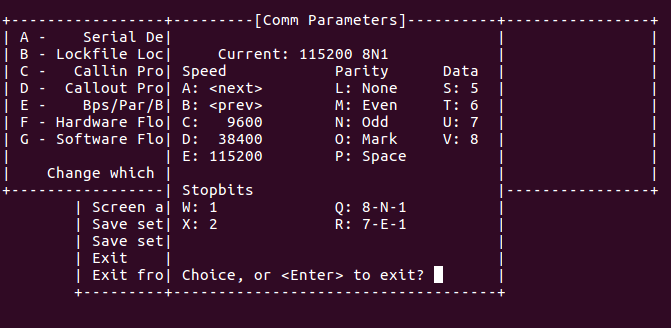
\includegraphics[width=\textwidth]{figs/baud-rate.png}
        \caption{Baud rate setting}
        \label{fig:baud}
    \end{subfigure}
    \label{fig:mini}
    \caption{Minicom printscrean during setup process}
\end{figure}
\paragraph{code}
The main code is similar to previous application using FreeRTOS. There is also an example on how to create and use a semaphore. There is still some trouble using semaphores, see \ref{sec:trouble}. To see how to set up USB port for the different MCU families, you can look at the file \emph{src/common.c}. The last useful function in the main file is \emph{$usb\_start()$}. This function creates the USB device structure, initialize two message queues, one for messages received and and one for sending messages and creates a FreeRTOS task called $usb\_task$. This task interacts with the USB device, polling every once in a while and sending messages when there are some to be send. The USB device created here is of type CDC (communication device class) and communicates exclusively with \emph{bulk} messages. More on information about the device creation can be found in \ref{chap:doc}.\newline
One of the tasks created in the main file is the \emph{adventure task}. This task is the adaptation of adventure (\cite{adventure}) entry point. This code wasn't written by us but retrieved from \cite{Gay2018} source code.\newline
All the USB relative functions are implemented in file \emph{src/usbcdc.c}. The important functions for this application are \emph{$usb\_getc$}, \emph{$usb\_getline$} and \emph{$usb\_printf$}. The first one gets a char from the host. It is a blocking function when there is nothing to be read. The second function gets an entire line from the host. It stops the reading when receiving a carriage return $"\backslash r \backslash n"$. The last function is similar to \emph{printf} c function, but uses the USB communication.
\section{USB-LED}
\label{sec:ul}
This last application is valid only for the stm32f3discovery board (figure \ref{fig:f3board}. This board contains 8 leds used in this project. The application is very simple, it use USB CDC device to drive the boards leds. There are 2 "functions" available for the user. One to select the leds to blink, one to select the blinking frequency.
\begin{itemize}
    \item "led $<leds>$", leds $\in \{LED0, LED1, ..., LED7\} $. Each different led must be separated by either a space or a comma. 
    \item "t $<time>$", blinking time, expressed in ms.
\end{itemize}
Either than that it is similar to the previous application. The reason for this application is to have a USB application written from scratch. This allowed us to spot some tricky part of the USB device implantation.
\begin{figure}
    \centering
    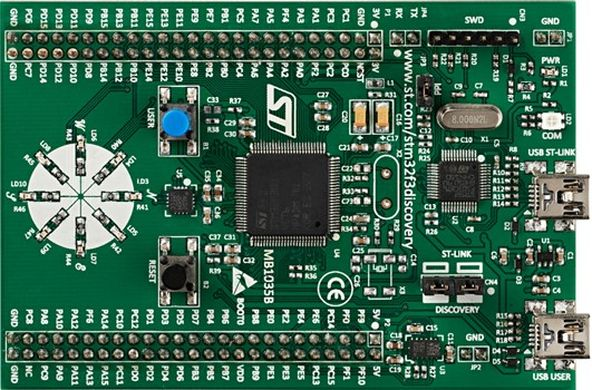
\includegraphics[scale=0.4]{figs/boardf3.jpg}
    \caption{f3 development board used in this appliation}
    \label{fig:f3board}
\end{figure}
\chapter{Documentation}
\label{chap:doc}
In this chapter we will give documentation about, the way to create a new project, the FreeRTOSConfig file used for this project, a description of the USB device structures as well as the code interfacing FreeRTOS with Libopencm3.\newline
To create a new project one need to run:
\begin{lstlisting}[language=bash]
$ make -f Project.mk PROJECT=PROJECT_NAME
\end{lstlisting}
For more information about FreeRTOS's configuration option visit\newline \href{https://www.freertos.org/a00110.html}{https://www.freertos.org/a00110.html}.
Important options are the following \ref{code:conf}:
\begin{itemize}
    \item Line 18: If set to 0 the RTOS uses cooperative scheduler. In this situation every task is assigned a timeslice of execution. In the preemptive mode, the scheduler runs the the task with the highest priority. If tasks have the same priority, the scheduler runs them in a cooperative mode. 
\paragraph{remark} When execution of a code doesn't seem to work, try to ensure that the priority of each task s correctly set. If a endless task has a high priority, none of the task with a lower priority will be executed.
    \item Line 23-27: In order to make the os softimers work correctly, we need to make the os aware of the MCU frequency. It is used internally by FreeRTOS for macros like $pdMS\_TO\_TICKS(time)$ converting a time value from ms to processor ticks. It is diffferent for f4 and f3 MCU as they don't run at the same frequency.
    \item Line 32-33: define the heap size. You need to make sure that you don't allocate more heap than the ram available on the controller.
    \item line 42: enabling the soft timers.
    \item line 58 and 60: Those two includes allows some function to be blocking. Take the example of receiving a message from a queue. If the flag $INCLUDE\_vTaskSuspend$ is set, then by passing argument $portMAX\_DELAY$ to the receiving function, the task is blocked if the queue is empty.
    \item The most important lines however are line 93 to 95. Those lines map the libopencm3 interrupt function to the FreeRTOS interrupt functions. This is used with \ref{code:cm3} to interface Libopencm3 and FreeRTOS. 
\end{itemize}
The last important file is \ref{code:usb}. This file contains everything relative to USB. For example one can see the structure defining the \emph{device descriptor} (line 28-43) and the \emph{configuration descriptor} (line 159 to 169). All information about the different structures can be found in \cite{usbNutshell}. The important functions, in order to initialize a USB device, in this file are the following:
\begin{itemize}
    \item line 230: This function is called when the device is plugged in a host's port. It initializes the different endpoints with their callback function and set the control callback function of endpoint 0.
    \item line 206: defines the rx (receiving message) handler. This function is called whenever a packet is received from the host. This function puts every received character into a message queue, which can later be retrieved by another task.
    \item line 274: Creates the message queues to send and receive USB packets. It also initialize the device and set the configuration callback. Finally, it creates a task that drives the USB device as explained in \ref{sec:ar}.
\end{itemize}
To find more information about the USB.org defined class you can visit \cite{usbClass}.
\chapter{Conclusion}
This project met the requirements, we used FreeRTOS along with Libopencm3 to implement a USB communication with a servo motor. We implemented a basic Makefile  project allowing us to easily create a new project using FreeRTOS and Libopencm3. Finally with the mean of this project, we provide to the uLiege robocup team a good tutorial to build a USB device. 
\label{chap:concl}
\section{Troubleshooting}
\label{sec:trouble}
We had some dig difficulties combining FreeRTOS with Libopencm3. This is mainly due to the different interrupt name functions. This is fixed thanks to the file $opencm3.c$ included in every project using FreeRTOS and Libopencm3. This solution was found in \cite{Gay2018}'s work.\newline
We also had some difficulties using semaphores. They seam to work fine when used inside a single task but not when shared accros different tasks. You can try this out with the application $semphr-test$. This was not considered as urgent for this project and is left for future work.
\section{Future work}
\label{sec:future}
The following work should tackle different problems.\newline
First handle semaphores across different task.\newline
Try to implement some software on a the actual servo board. This will allow us to try different functionalities such as the PWM module or the ADC and DAC converters. We will thus have a basic software allowing us to drive the robot's servo motors. A first step towards a working platform.\newline
Try to implement ISR with Libopencm3 and FreeRTOS.\newline
Think about the different class that might be more useful for our device and try out different type of USB message and study their performances depending on our needs. 
\begin{appendices}
This appendix contains some part of the code used in this project. However most of the file are just partially showed here. The reader might prefer to read from the source file.
\chapter{Code}
\section{Blink-led}
\lstinputlisting[language=C, caption={blink led}, label={code:blink}]{code/blink.c}
\lstinputlisting[language=C, caption={First FreeRTOS Task}, label={code:t1}]{code/task.c}
\section{Blink-led-RTOS}
\lstinputlisting[language=C, caption={blink-led-RTOS main}, label={code:m1}]{code/bRTOS.c}
\lstinputlisting[language=C, caption={Communication between tasks}, label={code:t2}]{code/t2.c}
\section{Queue-RTOS}
\lstinputlisting[language=C, caption={queue-led-RTOS main}, label={code:m2}]{code/qRTOS.c}
\section{Documentation}
\lstinputlisting[language=C, caption={FreeRTOS config}, label={code:conf}]{code/FreeRTOSConfig.h}
\lstinputlisting[language=C, caption={Opencm3.c}, label={code:cm3}]{code/opencm3.c}
\lstinputlisting[language=C, caption={USB device}, label={code:usb}]{code/usbcdc.c}

\end{appendices}
\bibliography{references} 
\bibliographystyle{apalike}
\end{document}
